% Worst-of autocallable notes priced against their disclosed estimated values.
%
% Layout follows the author's previous working paper: 11pt letterpaper article,
% 1in margins, newtx (Times), running head, booktabs tables with a note block
% under each. Two deliberate departures from that template are recorded at the
% points where they occur: the bibliography is APA author-date rather than the
% journal style used there, and the author block is single-author.
%
% Build: latexmk -pdf main.tex   (pdflatex + bibtex; biber is not required)
% The bibliography is generated, not written: see scripts/make_bibliography.py.

\documentclass[11pt,letterpaper]{article}
\usepackage[margin=1in,headheight=14pt]{geometry}
\usepackage[T1]{fontenc}
\usepackage[utf8]{inputenc}
\usepackage{amsmath,amsthm}
\usepackage{newtxtext,newtxmath}
\usepackage{microtype}
\usepackage{graphicx,booktabs,tabularx,array,multirow}
\usepackage{caption}
\usepackage{enumitem}
\usepackage{setspace}

% Departure from the previous paper, which used natbib with a hand-written
% journal-style bibliography. apacite with the natbibapa option keeps the
% \citep and \citet commands that template relies on while rendering the
% reference list in APA author-date form.
\usepackage[natbibapa]{apacite}

\usepackage{xurl}
\usepackage[hidelinks]{hyperref}
% xurl allows a break at every character and inserts stretchable glue at each
% one, so a justified line containing the repository URL opened a gap at its
% hyphen and read as "soham -parundekar". The glue is removed and the break
% points restricted to separators no reader would mistake for address
% characters. Both have to be set after xurl's own begin-document hook, which
% would otherwise put its defaults back.
\AtBeginDocument{%
  \Urlmuskip=0mu plus 0mu%
  \def\UrlBreaks{\do\/\do\.\do\=\do\?\do\&\do\_}%
  \def\UrlBigBreaks{\do\:}}
\usepackage{fancyhdr}
\usepackage{placeins}
\usepackage{etoolbox}

\providecommand{\SohamLocation}{\textit{India}}

\hypersetup{%
  pdftitle={Can the issuer's estimated value be reproduced from public data?
            Evidence from worst-of autocallable notes},
  pdfauthor={Soham Abhay Parundekar},
  pdfsubject={Independent repricing of 424B2 worst-of autocallable notes from public data},
  pdfkeywords={structured notes, autocallable, estimated value, local volatility,
               SVI, Longstaff-Schwartz, 424B2}}

\setstretch{1.06}
\setlength{\parindent}{1em}
\setlength{\parskip}{3pt}
\setlength{\emergencystretch}{2em}
\clubpenalty=10000
\widowpenalty=10000
\setlength{\textfloatsep}{13pt plus 3pt minus 3pt}
\setlength{\floatsep}{11pt plus 2pt minus 2pt}
\captionsetup{font=small,labelfont=bf,labelsep=period,justification=raggedright,
              singlelinecheck=false,skip=7pt}
\setcounter{topnumber}{2}
\setcounter{totalnumber}{3}
\renewcommand{\topfraction}{0.90}
\renewcommand{\textfraction}{0.08}
\renewcommand{\floatpagefraction}{0.80}

\pagestyle{fancy}
\fancyhf{}
\fancyhead[L]{\footnotesize Reproducing the issuer's estimated value}
\fancyfoot[C]{\thepage}
\renewcommand{\headrulewidth}{0.25pt}

\newcolumntype{Y}{>{\raggedright\arraybackslash}X}
\newcommand{\E}{\mathbb{E}}
\newcommand{\Var}{\operatorname{Var}}
\newcommand{\diag}{\operatorname{diag}}
\newcommand{\ind}{\mathbf{1}}
\newcommand{\F}{\mathcal{F}}
% Objects specific to this paper.
\newcommand{\worst}{W}                        % worst performance across underlyings
\newcommand{\lv}{\sigma_{\mathrm{LV}}}        % Dupire local volatility
\newcommand{\totvar}{w}                       % total implied variance
\newcommand{\logm}{k}                         % log-moneyness
\newcommand{\spread}{s}                       % funding spread over Treasuries
\newcommand{\notetext}[1]{\vspace{4pt}\par\noindent{\footnotesize\raggedright #1\par}}

\newtheorem{proposition}{Proposition}
\newtheorem{remark}{Remark}
\renewcommand{\arraystretch}{1.12}

\begin{document}

\thispagestyle{plain}
\begin{center}
{\LARGE\bfseries Can the issuer's estimated value be reproduced\\from public data?\par}
\vspace{7pt}
{\large Evidence from worst-of autocallable notes\par}
\vspace{14pt}

{\fontsize{10.1}{11.7}\selectfont\bfseries Soham Abhay Parundekar\par}
\vspace{1.5pt}
{\fontsize{8.0}{9.4}\selectfont\href{mailto:parundekarsoham@gmail.com}%
  {\nolinkurl{parundekarsoham@gmail.com}}\par}
\vspace{1.0pt}
{\fontsize{8.5}{10.0}\selectfont Independent Researcher, \SohamLocation\par}
\end{center}
\vspace{8pt}

\begin{abstract}
% Written last, after every section is approved. Every figure in it must trace to the numeric evidence ledger.
\noindent
US structured note issuers print an estimated value on the cover of every
pricing supplement, computed with models and a funding rate the filing does not
disclose. This paper asks whether an outside party can reproduce that figure,
and tests the question on the hardest instrument it covers: worst-of
autocallable notes on three correlated equity indices, whose redemption before
maturity is the issuer's to initiate rather than automatic on five of the six
notes studied. Surfaces
are fitted to public option quotes under no-arbitrage constraints, converted to
local volatility, and simulated jointly, with the issuer's call solved by
least-squares Monte Carlo from the issuer's side of the contract.

The disclosed figure is not reproduced. Independent valuations land below it on
all six notes, by \$11.41 to \$27.92 per \$1{,}000 of principal across the five
whose barriers are covered by quoted strikes, against simulation standard
errors below \$0.40. Solving for the funding spread that would reconcile the
two valuations returns a negative spread on every note, from $-278$ to $-123$
basis points against an A-rated corporate benchmark of 69, so the undisclosed
funding rate cannot account for the difference. Four further candidates are
excluded on direction or magnitude. Two survive, the correlation assumption and
the shape of the volatility surface, and a third, the dynamics of that surface,
lies outside what a local-volatility model can test; none of the three is
published in the filings. A
census of the same week bounds the exercise: of 1{,}086 supplements filed, 129
are final notes of this type, and 71 of those can be priced from public quotes
at all.

\end{abstract}

\noindent\textit{Keywords:} structured notes; autocallable; estimated value;
local volatility; Monte Carlo.\par
\noindent\textit{JEL classification:} G12, G13, G14, G24.
\vspace{8pt}

\section{Introduction}\label{sec:intro}
% Objective: State the question, the answer (no), and the two contributions: the verification result on six notes, and a census of what is priceable at all.

The cover page of a US structured note's pricing supplement carries an estimated
value: the issuer's own figure for what the security is worth, set below the
price the investor pays for it. One of the notes examined here was sold at
\$1{,}000 and disclosed at \$938.90. The practice traces to a sample comment
letter from the SEC's Division of Corporation Finance \citeyearpar{SEC2012},
which asked issuers to ``consider prominently disclosing'' such a figure; it is
staff guidance and not a rule, and no rule has since replaced it. What the filing
omits is how the number was reached. The model belongs to the issuer, so does
the volatility surface, and the discount curve embeds an internal funding rate
that appears nowhere in the document. An investor is given a valuation and no
means of checking it.

This paper asks whether the figure can be reproduced from outside the issuer,
using only public data.

The question is put to worst-of autocallable notes, which are the most
demanding instrument in the disclosure rather than the most convenient. Payment
tracks the weakest of three correlated equity underlyings. A contingent coupon
is paid only when every leg closes at or above its barrier on an observation
date, and principal is returned in full only if the weakest leg finishes above
a lower trigger. The call deserves particular attention, because the product's
name misdescribes it. On five of the six notes priced here redemption is not
automatic: three are redeemable at the issuer's option, and two are redeemed,
in the issuer's own words, ``if and only if the output of a risk neutral
valuation model \ldots\ indicates that redeeming on such date is economically
rational for us.'' Only one note in the sample redeems mechanically when a
level is reached. Valuing any of them calls for a joint model that carries each
leg's skew, a correlation structure, and an exercise rule solved from the
issuer's side of the contract, where the holder of the option is short the
investor's payoff and stops to minimise it.

Every input is public. Implied volatility surfaces are fitted to delayed
end-of-day option quotes from Cboe under the no-arbitrage conditions of raw
SVI, converted to Dupire local volatility, and simulated jointly against a
Treasury discount curve; the issuer's call is solved by Longstaff--Schwartz
regression on 200{,}000 paths. Before any note is priced the engine is made
to return the vanilla prices it was calibrated to, measured against the quoted
bid-ask width rather than in isolation, since an error only counts as large
relative to the price uncertainty of the market it came from. Four of the five
surfaces return a median error below 0.26 of the quoted bid-ask width, well
inside the band the market itself prices in. The S\&P 500 surface does not, and
\S\ref{sec:validation} attributes that to its exceptionally narrow quoted width
rather than to a poor fit: at 0.131 volatility points its absolute error falls
inside the range the other four surfaces span, while its quoted width is 4.7
times narrower than the next tightest in the sample.

The answer is no. On all six notes the independent valuation lands below the
disclosed figure, by \$11.41 to \$27.92 per \$1{,}000 of principal across the
five notes whose barriers are covered by quoted strikes, or 1.17 to 2.97 per
cent of the disclosed value. Inverting the question makes the size of the
problem clearer: solving for the constant funding spread over Treasuries that
would set model value equal to disclosed value returns a negative spread on
every note for which the solution brackets, from $-278$ to $-123$ basis points,
against an option-adjusted spread of 69 basis points on A-rated US corporate
debt on the pricing date. Reconciliation would require the issuer to borrow
below the Treasury curve. A funding rate the filing does not disclose is
therefore not a sufficient explanation for the difference, which is the
candidate a reader would reach for first.

What follows from this is narrower than it may appear, and the limits are worth
stating before the evidence. The result is not a finding of overpricing.
\citet{Henderson2011} established that these notes are issued above model
value, and the disclosed estimated value is itself below the issue price, so
both orderings already hold; the gap measured here is between the disclosed
value and an independent valuation, not between either and the price. Nor does this paper
identify what the residual is made of, though it narrows the field.
\S\ref{sec:inputs} takes the candidates one at a time and excludes four of
them: funding and observation timing move the value the wrong way, while the
proxied leg and the term extrapolation move the right way by too little or on
too few notes. Suboptimal exercise accounts for part of three notes and is
arithmetically unavailable for two. Two measured candidates survive, the
correlation assumption and the shape of the volatility surface, and a third,
the dynamics of that surface, is one a local-volatility model cannot test at
all. None of the three is published in the filings. Which is at work, or in
what combination, is not something six notes can settle. Six notes from
one week support a bounded claim and no population statement.

Two contributions remain. The first is the verification exercise itself, run on
the product class the nearest published work set aside: \citet{Bauer2020} check
issuer-disclosed values against standard option pricing models on German retail
certificates and state plainly that ``[m]ore complex products like
autocallables are left for future research.'' This paper prices them, and
reports the funding-spread inversion as a diagnostic that converts an
unexplained difference into a statement about what the difference cannot be.
The second is a census of what any such exercise can reach. Of 1{,}086
prospectus supplements filed on Form 424B2 in a single week, 129 are final
worst-of notes with a contingent coupon and a disclosed estimated value, and 71
of those, 55 per cent, can be priced from public option quotes at all. The
remainder reference underlyings with no listed options or no usable chain. Any
outside verification of this disclosure is bounded by that fraction, and
\S\ref{sec:data} reports where the rest of the market goes.

\section{The disclosed estimated value, and prior work}\label{sec:prior}
% Objective: What the number is and where it comes from: SEC staff guidance, not a rule. Position against Bauer et al., who verified such values on German certificates and left autocallables to future research.

\subsection{What the issuers say the number is}

The filings are explicit that the estimated value is a model output and whose
model it is. One of the supplements priced here states that the issue price
``exceeds the estimated value of your notes as of the time the terms of your
notes are set on the trade date, as determined by reference to GS\&Co.'s
pricing models and taking into account our credit spreads,'' and that those
``pricing models are proprietary and rely in part on certain assumptions about
future events, which may prove to be incorrect.''\footnote{Quotations in this
subsection are from the pricing supplement for note N4, filed by GS Finance
Corp.\ under accession number 0001193125-26-419171 and preserved in full in the
project repository; the filings for all six notes are identified in
Appendix~\ref{app:terms}. The other three issuers in the sample describe the
figure in materially similar terms, each naming its own proprietary models:
Morgan Stanley's supplements say the estimated value ``is determined using our
own pricing and valuation models'' and that these ``are proprietary,'' and
BofA's say it is ``determined as of the pricing date by reference to our and
our affiliates' pricing models.''} The same document lists the inputs: ``our credit spreads, interest rates (forecasted, current and
historical rates), volatility, price-sensitivity analysis and the time to
maturity of the notes.''

That list is worth reading closely, because correlation does not appear in it.
The note it describes pays on the weakest of three equity indices, and
\S\ref{sec:results} shows the investor is long correlation on every note in the
sample. Morgan Stanley's supplements list their inputs too, naming ``market inputs and
assumptions relating to the underliers, instruments based on the underliers,
volatility and other factors including current and expected interest rates,''
and correlation is absent there as well. Both lists are introduced as partial,
with ``including principally'' and ``other factors,'' so neither purports to be
complete and no inference follows that either model ignores correlation. What does follow is narrower and is the point of this paper: the
disclosure names the inputs it considers principal, and the input that most
distinguishes a worst-of structure from a single-underlying one is not among
them.

The gap between the issue price and the estimated value is itself attributed,
in the same document, to ``the underwriting discount and commissions, the
expenses incurred in creating, documenting and marketing the notes, and an
estimate of the difference between the amounts we pay to GS\&Co.\ and the
amounts GS\&Co.\ pays to us in connection with your notes.'' The first two
components appear on the cover as numbers. The third does not. It is the
internal transfer between the issuing entity and its distribution affiliate,
and it is the component that the phrase ``internal funding rate'' is usually
reaching for. That phrase belongs to the issuers rather than to the guidance. The 2012
comment letter discussed below does not contain it, while JPMorgan's supplements
in this sample carry a risk factor headed ``Estimated Value of the Notes Is
Derived by Reference to an Internal Funding Rate.'' The attribution matters
because the rate it names is the one input a reader cannot recover.

One further sentence in the same risk factor deserves attention, since it
anticipates this paper's exercise and declines to bound it. The actual value an
investor could realise ``may differ, perhaps materially, from the estimated
value of your notes determined by reference to our models due to, among other
things, any differences in pricing models or assumptions used by others.'' The
filing therefore tells the reader that another party's model may disagree, by
an amount it does not characterise, for reasons it does not enumerate. Putting
a number on that disagreement for a specific class of notes, from inputs the
reader can obtain, is what follows in \S\ref{sec:results}.

\subsection{Where the disclosure comes from}

The practice originates in an April 2012 sample comment letter from the
Division of Corporation Finance, addressed to financial institutions issuing
structured notes \citep{SEC2012}. On the valuation figure the letter asks that
issuers ``should consider prominently disclosing'' it, language that is
advisory in form as well as in effect. A sample comment letter is staff
guidance: it conveys the views of the staff, not a rule adopted by the
Commission, and it binds no one. No rule has since replaced it for this figure.

The practical consequence is that there is no prescribed form, and the sample
examined here shows the range that permits. Among the final worst-of
contingent-coupon supplements filed in the sample week, five carry no point
estimate in the filed document. Three state the figure as a bound rather than a
number, with the cover reading ``Our estimated value of the notes on trade
date: Not less than the face amount of such notes.'' The remaining two carry
only the risk-factor heading and locate the figure in an accompanying index
supplement that is not part of the document filed under the
cover.\footnote{These five supplements are not among the six priced here and
are therefore not preserved in the project repository, which holds only the
documents the valuations depend on. They remain retrievable from EDGAR under
accession numbers 0001193125-26-415466, 0001193125-26-413990 and
0001193125-26-413989 for the three quoting a bound, and 0000950103-26-015173
and 0000950103-26-015172 for the two deferring to a supplement.} All five
come from one issuer. None of this is a deficiency, since nothing requires a
point estimate; it is what discretionary disclosure looks like when it is
exercised.

The timing is constrained even where the content is not. Rule 424(b)(2)
requires the priced supplement to be filed no later than the second business
day following the earlier of the date of determination of the offering price or
the date it is first used \citep{SEC424b2}. A verification exercise therefore
has a short and known window in which the terms are fixed and public, which is
what makes a single week a coherent sample rather than an arbitrary one.

\subsection{Prior work}

The literature on retail structured products has measured issuer margins for
two decades, mostly in Europe and mostly by replication. \citet{Wilkens2003}
document premia over replication cost and a life-cycle pattern in German
products; \citet{Stoimenov2005} extend the fair-pricing analysis across
equity-linked retail instruments; \citet{Entrop2016} quantify overpricing of
discount certificates and attribute a substantial share of it to issuer credit
risk; and \citet{Ruf2011} relates pricing power to credit quality. In the US,
\citet{Henderson2011} is the canonical study, establishing that these notes are
issued above model value, and \citet{Deng2011} give an early valuation
treatment of autocallable structures alongside evidence of their growth. The
methods for valuing the structures themselves are well developed:
\citet{Guillaume2015} derives analytical results covering memory coupons,
partial protection and worst-of contingencies, and \citet{Kim2019} construct
static replications of autocallable and barrier features as an alternative to
simulation.

This paper differs from all of these in its object. They measure the distance
between a price and a model value. The question here is the distance between
two model values, one of which the issuer published. The nearest precedent for
treating a disclosed figure as the thing under examination is
\citet{Jorgensen2011}, who compare overpricing against costs the issuer
disclosed at issuance and find roughly half of it unexplained. On the US
estimated-value disclosure specifically, \citet{Lai2022} assembles a large
EDGAR sample of auto-callable reverse convertibles, but studies realised
returns rather than whether the disclosed figure can be reproduced.

The closest published work is \citet{Bauer2020}, who check issuer-disclosed
fair values against standard option pricing models for German retail
certificates and conclude that the disclosed values can be reproduced. Their
sample is of simpler instruments, and they say so: ``[m]ore complex products
like autocallables are left for future research.'' Three features of the setting
examined here make that an unusually clean gap to occupy. The product is a
worst-of on several correlated underlyings rather than a single one. On five of
the six notes redemption before maturity is not automatic, three being at the
issuer's option and two following the disclosed rational-exercise rule quoted
in \S\ref{sec:intro}, so valuation requires an optimal-stopping problem solved
against the investor rather than a barrier check. And the figure rests on staff
guidance that prescribes neither a method nor a form, which is what makes
reproducing it a question about the disclosure and not only about the model.
Whether a disclosed value can be reproduced is therefore open in this market
rather than settled elsewhere and carried across.

\section{Sample and data}\label{sec:data}
% Objective: The calendar constraint from Rule 424(b)(2); the screening census; the six notes and the structures they span.

\subsection{Why the sample is one week}

A note can only be repriced against its disclosed value while its terms are
both fixed and public, and that state begins later than one might expect and is
announced only briefly. The preliminary supplement carries ranges: a coupon quoted as
``at least'' some rate, a trigger to be determined, an estimated value given as
an interval.\footnote{The phrasing is standard across the preliminary
supplements in this week. One example, filed under accession number
0001918704-26-031175, offers ``a Contingent Interest Rate of at least 9.70\%
per annum.'' These documents are superseded by their priced counterparts and
are not preserved in the repository.} The priced supplement replaces all of it with numbers, and Rule
424(b)(2) requires that document to be filed no later than the second business
day following the earlier of the date the offering price was determined or the
date the supplement is first used \citep{SEC424b2}.

So the terms arrive in a stream of final supplements with a two-day lag and no
subsequent amendment. Choosing a calendar week and taking every qualifying
filing in it is therefore a sampling rule a reader can check, and one that
cannot be tuned after the fact by extending the window until the results
improve. The week used here is 5 to 9 October 2026. Five of the six notes were
priced on 7 October and the sixth on 5 October.

\subsection{What the week contained}

% Generated by scripts/make_paper_tables.py from the frozen results.
% Do not edit by hand; the next build overwrites it.
\begin{table}[tbp]
\centering
\caption{Every 424B2 filed in the pricing week, by the reason it does or does not reach the sample}
\label{tab:census}
\small
\begin{tabular}{l r r}
\toprule
Disposition & Filings & Share (\%) \\
\midrule
Preliminary supplement; terms not yet fixed & 667 & 61.4 \\
Not a worst-of structure & 201 & 18.5 \\
No contingent coupon & 84 & 7.7 \\
No estimated value disclosed & 5 & 0.5 \\
Single-name or fund underlyings & 16 & 1.5 \\
An underlying with no listed options & 42 & 3.9 \\
Priceable from public option quotes & 71 & 6.5 \\
\midrule \textit{Total 424B2 filings} & \textit{1,086} & \textit{100.0} \\
\bottomrule
\end{tabular}
\notetext{\textit{Notes:} All 424B2 filings retrieved from EDGAR full-text search for the week of the snapshot. Each filing is assigned to the first stage it fails, so the rows partition the population. A preliminary supplement is excluded because its coupon, trigger and estimated value are still ranges. The last three rows are the final worst-of notes with a contingent coupon and a disclosed estimated value, 129 in all, of which 71 (55\%) can be priced from public option quotes; the six notes studied here are drawn from those 71. Source: \texttt{src/data/edgar\_notes.py}.}
\end{table}


Table~\ref{tab:census} is the whole filing population, each filing assigned to
the first stage it fails, so the rows partition rather than overlap. Of 1{,}086
supplements filed on Form 424B2 that week, 667 are preliminary and 285 are
final but not the structure under study, either because they are not worst-of or
because they carry no contingent coupon. A further five are final worst-of notes
with a contingent coupon that state no point estimate of the value, discussed
in \S\ref{sec:prior}.

That leaves 129 final worst-of contingent-coupon notes with a disclosed
estimated value, of which 71 can be priced from public option quotes. Of the 58
that cannot, 16 are written on single names or funds and 42 carry at least one
leg whose options are not listed. That second group is more concentrated than
one would guess. In 33 of the 42 the only such leg is the Nasdaq-100 Technology
Sector index, a US index with no options market of its own; the remaining nine
reference the EURO STOXX 50, the Nikkei 225 or a futures-based Russell variant.
The ratio is worth carrying forward. An outside party attempting this
verification can reach 55 per cent of the qualifying market, and what it cannot
reach is not a random sample of the rest but is dominated by notes on a
single index that has no options market of its own.

\subsection{The six notes}

% Generated by scripts/make_paper_tables.py from the frozen results.
% Do not edit by hand; the next build overwrites it.
\begin{table}[tbp]
\centering
\caption{The six notes: underlyings, terms and the figures the issuer discloses}
\label{tab:terms}
\small
\begin{tabular}{l l l r r r r r r}
\toprule
Note & Issuer & Underlyings & Tenor & Coupon & Barrier & Trigger & Est.\ value & Commission \\
\midrule
N1 & JPMorgan & NDX, RUT, SPX & 5.00 & 8.30 & 70.00 & 65.00 & 938.90 & 41.25 \\
N2\textsuperscript{a} & Morgan Stanley & DJX, NDX, RUT & 5.00 & 8.30 & 70.00 & 65.00 & 943.10 & 36.25 \\
N3 & Morgan Stanley & NDX, RUT, SPX & 3.01 & 9.75 & 70.00 & 60.00 & 983.40 & 2.50 \\
N4 & Goldman & NDX, RUT, SPX & 1.92 & 10.15 & 65.00 & 60.00 & 999.00 & 5.25 \\
N5 & BofA & NDX, RUT, SPX & 1.75 & 6.25 & 75.00 & 70.00 & 972.10 & 25.00 \\
N6 & JPMorgan & RUT, SPX, SMH & 1.92 & 12.40 & 65.00 & 60.00 & 967.30 & 22.25 \\
\bottomrule
\end{tabular}
\notetext{\textit{Notes:} Tenor in years from pricing date to stated maturity. Coupon is the contingent rate per annum in per cent, paid only when every underlying is at or above its coupon barrier on an observation date. \textit{Barrier} is that coupon threshold and \textit{Trigger} the principal-repayment threshold, both as a percentage of the initial level. Estimated value and selling commission are per \$1,000 of principal, as disclosed in the pricing supplement. \textsuperscript{a}\,Held out of the ranges quoted in the text: no fitted slice past one year carries a quoted strike at this note's trigger on one leg, so its downside is extrapolated rather than observed. Source: the filings listed in Appendix~\ref{app:terms}.}
\end{table}


Six of the 71 are priced here, listed in Table~\ref{tab:terms}, chosen to span
the structural variation rather than to be representative in any statistical
sense. They come from four issuers. Tenors run from 1.75 to 5.00 years, contingent
coupons from 6.25 to 12.40 per cent per annum, coupon barriers from 65 to 75
per cent of the initial level and downside triggers from 60 to 70 per cent. The
disclosed estimated values run from \$938.90 to \$999.00 per \$1{,}000 and the
selling commissions from \$2.50 to \$41.25, the low figure belonging to a note
sold only into fee-based advisory accounts where the adviser is compensated
separately.

The call mechanics vary more than the name of the product suggests, and the
variation is the reason six notes are enough to be interesting. Three are
redeemable at the issuer's option on scheduled dates. Two redeem under the
disclosed rational-exercise rule quoted in \S\ref{sec:intro}. One, and only
one, is auto-callable in the ordinary sense: redemption is mechanical when every
underlying closes at or above 93.25 per cent of its starting level on one of
six observation dates. That threshold is itself worth noting, since discussions
of these products often assume the automatic call sits at the initial level.

\subsection{Option data and the fitted surfaces}

Implied volatility surfaces are fitted to delayed end-of-day option chains
retrieved from Cboe's public endpoint and preserved as of 9 October 2026, with a
SHA-256 digest recorded for every file. Five surfaces cover the eighteen leg positions the six
notes carry between them, which resolve to five distinct underlyings. Expiries inside a fortnight are dropped, as are quotes whose
relative bid-ask exceeds 0.35, and log-moneyness is clipped to $[-0.9, 0.45]$;
consecutive expiries closer than 25 days apart are thinned so that the calendar
condition is tested across separated maturities rather than across
adjacent weeklies.

Each slice's forward and discount factor come from a put-call parity regression
across near-the-money strikes. Three of the five surfaces are fitted to cash
index options, which are European, and for these both quantities are fitted.
The other two are fitted to exchange-traded fund options, which are American,
and there the discount factor is pinned to the Treasury curve and only the
forward is fitted. Parity is an identity only under European exercise: left to
fit freely on the semiconductor ETF, the regression returned a discount factor
implying a 1.6 per cent zero rate against 4.3 per cent Treasuries, because the
early-exercise premium on in-the-money puts grows with strike and tilts the
slope. Pinning the discount factor removes that tilt while leaving the forward
to carry the market's dividend assumption. Near the money the early-exercise
premium itself is small enough to leave in the quotes, which is an
approximation rather than a correction and is revisited in \S\ref{sec:limits}.

\subsection{The one proxied leg}

Four of the five underlyings are priced off options on the instrument named in
the term sheet. The exception is the Dow Jones Industrial Average, whose listed
index options are too sparse to fit a surface across the maturities these notes
need, and which is therefore priced off options on the ETF that tracks it.

What that substitution costs can be measured rather than assumed, because two
other legs in the sample have both an index and an ETF chain available at shared
expiries. At-the-money implied volatility is higher on the fund than on the
index in every comparison: by 0.517 volatility points for the Dow pair at the
one expiry they share, and by 0.434 and 0.435 points on average for the
Nasdaq-100 and Russell 2000 pairs across 16 shared expiries each, reaching
beyond one and two years respectively. The sign is consistent and the magnitude
is similar across all three, which is what makes the Dow figure usable as an
estimate rather than a single observation.

Correcting that one leg, and nothing else, shifts the affected note's value from
\$893.93 to \$896.54, a rise of \$2.61 with a standard error of \$0.73, and
narrows its difference from the disclosed value from \$49.17 to \$46.56. The
proxy therefore accounts for about five per cent of that note's gap and moves it
in the direction that would close it. It is the same note whose downside trigger
falls outside the quoted strike range on the Dow leg, which is why
\S\ref{sec:results} reports it but holds it out of the stated ranges;
Appendix~\ref{app:coverage} gives the coverage counts leg by leg.

\subsection{Rates, spreads and the volatility indices}

Discounting uses the US Treasury par yield curve for the valuation date, as
published by the Treasury. The benchmark against which an implied funding spread
is judged is the ICE BofA A-rated US corporate index option-adjusted spread,
69 basis points on the pricing date, taken from the Federal Reserve Bank of St
Louis. The Cboe volatility indices for the S\&P 500, Nasdaq-100 and Russell
2000 supply the surface move between the pricing date and the snapshot date used
in \S\ref{sec:inputs}, each index matched to the leg it measures. Daily closes
for the semiconductor ETF come from a commercial endpoint rather than an
official series, no free official source for a single fund's history being
available; that series affects one note of the six.

Every series above is free and unauthenticated, and the retrieval code is in the
repository. The option chains the reported results depend on are preserved with
their digests, since a delayed-quote endpoint serves only current quotes and the
9 October snapshot cannot be retrieved again.

\section{Method}\label{sec:method}
% Objective: Quotes to forwards to SVI under arbitrage constraints, Dupire local volatility, correlated multi-asset simulation, Longstaff-Schwartz for the issuer's call, and the funding-spread inversion.

\subsection{The volatility surface}

Each expiry is fitted separately in total implied variance against
log-moneyness, $\totvar(\logm) = \sigma_{\mathrm{BS}}^2(\logm)\,T$ with
$\logm = \ln(K/F_T)$, using the raw SVI parameterisation of
\citet{GatheralJacquier2014},
%
\begin{equation}
  \totvar(\logm) = a + b\left[\rho\,(\logm - m)
      + \sqrt{(\logm - m)^2 + s^2}\,\right].
  \label{eq:svi}
\end{equation}
%
Fitting variance rather than volatility is a choice the next step forces. Local
volatility needs $\partial\totvar/\partial T$ and
$\partial^2\totvar/\partial\logm^2$, and \eqref{eq:svi} is twice differentiable
in $\logm$ in closed form, so those derivatives come off a fitted slice instead
of off differenced quotes.

Two arbitrage conditions are imposed, both from \citet{GatheralJacquier2014}.
The risk-neutral density implied by a slice is non-negative exactly when
%
\begin{equation}
  g(\logm) = \left(1 - \frac{\logm\,\totvar'}{2\totvar}\right)^{\!2}
    - \frac{(\totvar')^2}{4}\left(\frac{1}{\totvar} + \frac14\right)
    + \frac{\totvar''}{2} \;\geq\; 0
  \label{eq:butterfly}
\end{equation}
%
everywhere, and total variance must not decrease in $T$ at fixed $\logm$, or a
calendar spread prices negative. Neither check is cosmetic. A slice violating
\eqref{eq:butterfly} has negative density somewhere, and the denominator of the
local-variance expression below passes through zero at that point, which is the
usual reason a local-volatility surface comes back full of undefined values.
When a check fails the slice is refitted subject to the constraint rather than
repaired afterwards, the arbitrage-free parameter domain being characterised by
\citet{MartiniMingone2022}.

Where the conditions are enforced turns out to matter as much as whether they
are. Checking on one fixed wide grid asks a two-week slice about strikes far
below its deepest quote, where it is purely extrapolating, and enforcing the
calendar condition out there makes each short-dated slice's extrapolated
wing a floor for the next expiry, so the constraint propagates forward from the
slice carrying the least information rather than the most. The grid is scoped
to the strikes each pair of adjacent expiries actually quotes, padded slightly
and capped at five standard deviations of total volatility. Quotes enter the fit
only if the expiry is at least a fortnight out and the relative bid-ask is at
most 0.35, with log-moneyness clipped to $[-0.9, 0.45]$, and consecutive
expiries closer than 25 days apart are thinned so that the calendar condition
is tested across separated maturities rather than adjacent weeklies. The
surfaces retain between 11 and 20 fitted slices each.

\subsection{Local volatility}

The simulation diffusion is Dupire local volatility, taken in Gatheral's
log-moneyness form,
%
\begin{equation}
  \lv^2(\logm, T) = \frac{\partial\totvar/\partial T}
    {1 - \dfrac{\logm}{\totvar}\dfrac{\partial\totvar}{\partial\logm}
      + \dfrac14\left(-\dfrac14 - \dfrac{1}{\totvar}
        + \dfrac{\logm^2}{\totvar^2}\right)
        \left(\dfrac{\partial\totvar}{\partial\logm}\right)^{\!2}
      + \dfrac12\dfrac{\partial^2\totvar}{\partial\logm^2}}.
  \label{eq:dupire}
\end{equation}
%
Derivatives in $\logm$ are exact. In $T$ the surface is interpolated linearly
in total variance between adjacent expiries, which makes
$\partial\totvar/\partial T$ piecewise constant but non-negative, because the
calendar condition already forced $\totvar$ to be non-decreasing in $T$. The
butterfly condition keeps the denominator of \eqref{eq:dupire} positive. Local
variance is therefore positive by construction rather than by inspection, which
is the reason the two checks in the previous subsection are not optional. The
implementation still counts how often it has to clamp, so a failure would be
visible rather than silent.

Past the longest listed expiry the surface must be extrapolated, and for the
five-year notes that is a long way. Quoted expiries reach 5.20 years on the
S\&P 500 but stop at 3.20 on the Nasdaq-100 and 2.19 on the Russell 2000, while
the two longest notes run to 5.00 years. The base case holds implied volatility
flat in maturity with its smile shape intact,
$\totvar(\logm,T) = \totvar_{\mathrm{last}}(\logm)\,T/T_{\mathrm{last}}$. Two
alternatives are implemented so the choice can be measured rather than
asserted: carrying the last observed variance slope forward, and shifting every
volatility by a fixed amount. \S\ref{sec:inputs} reports what the choice is
worth, which ranges from \$0.22 on the shortest note to \$12.36 on the longest.

\subsection{Correlation}

Correlation is estimated from 252 trading days of daily log returns, taken up to
and including each note's own pricing date rather than the snapshot date. Five
of the six notes priced two business days before the snapshot, so using
everything available would feed future returns into a historical pricing
decision; the effect on the matrix is small and the principle is not. Where the
sample matrix is not positive semidefinite, the nearest valid correlation matrix
in the Frobenius norm is substituted by the alternating-projection method of
\citet{Higham2002}.

This is the largest approximation in the method and it runs in a known
direction. Vanilla options carry no information about co-movement, and there is
no free source of implied correlation, so a realised estimate stands in for a
risk-neutral input. Dealers mark correlation above realised for precisely this
product, because selling a worst-of leaves the desk short correlation. The
investor is long correlation on every note in the sample, so if the issuer used
a higher figure than the one estimated here, its value would exceed this
paper's for that reason alone. That makes correlation the first candidate
\S\ref{sec:inputs} has to rule in or out, and the one it treats at most length.

\subsection{Simulation}

Paths are generated by daily log-Euler steps under the risk-neutral measure,
each asset drifting along its own forward curve so that carry is whatever the
option market implies rather than a separately assumed dividend yield, and
diffusing at \eqref{eq:dupire}. Shocks are correlated through the Cholesky
factor of the correlation matrix. Antithetic variates are used, which help most
where the payoff is discontinuous, and the reported figures use 200{,}000 paths.

Three implementation choices are worth recording because they decide what is
computationally possible rather than merely convenient. Paths are not stored: a
five-year note observed monthly needs 1{,}260 daily steps on three assets, and
retaining 200{,}000 of them would run to several terabytes, so the engine
carries only the current level and records at each observation date the
statistics the payoffs need, which are the worst and best performances across
underlyings. The American knock-in is handled by a running indicator updated
every day, since the condition it tests, that an underlying's value falls below
its threshold ``on any Trading Day during the Knock-In Period,'' cannot be
evaluated from the observation dates alone. That note's loss condition is a
conjunction rather than a single test: a knock-in must occur and the least
performing underlying must also finish below its starting value, not merely
below the threshold that triggered the knock-in. Local volatility is read from a precomputed grid in
$(\logm, T)$ with bilinear interpolation rather than evaluated analytically at
every step, which reproduces the surface to well under a basis point of
volatility and is what makes bump-and-revalue Greeks affordable. Common random
numbers come from re-seeding rather than from stored draws, so a bumped
revaluation differs from the base case only in the bumped input and each Greek
is a clean finite difference.

A European control variate is applied, with the variance reduction factor
running from 1.8 to 3.8 across the six notes. Standard errors on the reported
values fall between \$0.24 and \$0.37 per \$1{,}000.

\subsection{The issuer's call}

The Bermudan call is solved by least-squares Monte Carlo
\citep{LongstaffSchwartz2001}. Treating an issuer's early-redemption right as
an optimal-stopping problem rather than as a barrier test has published
precedent in this product family: \citet{Detemple2021} solve for the optimal
policy explicitly on callable barrier reverse convertibles, and
\citet{Huo2025} applies least-squares Monte Carlo to worst-of issuer-callable
notes of the kind priced here, under a multi-variate local-volatility model and
with the stopping problem posed from the issuer's side. One sign convention has
to be stated plainly, because reversing it would change every result. A high continuation
value is the issuer's liability, not its asset. The issuer therefore redeems
when keeping the note alive costs it more than repaying principal now, so the
investor's value at a call date is the redemption amount whenever the estimated
continuation value exceeds it. Solved the other way the issuer's option becomes
a gift to the investor and every price rises.

The regression basis is deliberately small: a constant, the worst performance
$\worst$, its square, the spread between best and worst performance, and
accrued-but-unpaid coupon. The worst performer is the state variable that drives
the payoff, and its square lets the exercise boundary curve; the best-worst
spread carries the dispersion a worst-of note is exposed to; accrued coupon
matters only where the note has a memory feature. A richer basis fits
simulation noise and estimates a worse boundary rather than a better one.

One detail of the comparison is easy to get wrong in the direction the term
sheets invite. A coupon due on a call date is paid whether or not the note is
redeemed, so it cancels from the decision and the continuation value is
compared against par alone. Term sheets quote the redemption as par plus
coupon, and carrying that wording into the comparison makes calling look about
one coupon more expensive than it is, which systematically under-calls and
overvalues the note.

\subsection{The funding-spread inversion}

The gap between a model value and the disclosed value can be expressed as the
discount-rate adjustment that would remove it. For a constant spread $\spread$
over the Treasury zero curve,
%
\begin{equation}
  V(\spread) = \E^{\mathbb{Q}}\!\left[\;\sum_i
    e^{-(r_{t_i} + \spread)\,t_i}\, \mathrm{CF}_i \right],
  \qquad
  \text{solve } V(\spread^\ast) = \mathrm{EV}_{\text{disclosed}} .
  \label{eq:inversion}
\end{equation}
%
The spread enters the exercise policy as well as the discounting, so
\eqref{eq:inversion} is solved by repricing on a fixed set of paths rather than
by rescaling a single valuation. $V$ is monotone decreasing in $\spread$, so the
root is bracketed and found by Brent's method.

What makes $\spread^\ast$ informative is that its sign is known in advance.
Discounting a liability at a wider spread lowers its value, and an issuer funds
above Treasuries, so a disclosed value derived with the issuer's own funding
rate should reconcile at a positive $\spread^\ast$. A negative solution cannot
be a funding spread. Because the issuer's call is the largest discretionary
input in the model, \eqref{eq:inversion} is solved under two assumptions about
it, optimal exercise and no early call, and \S\ref{sec:results} reports both.

\section{Validation}\label{sec:validation}
% Objective: What was checked before any note was priced, including the one honest failure and why it is a property of the SPX option market.

A note's value is not observable, so nothing downstream of the pricing engine
can be checked against a market. Everything upstream can be, and is, because a
model that cannot return the instruments it was calibrated to has no claim on
the instrument it was built for. This section reports those checks in the order
the pipeline runs them, including the one that does not pass.

\subsection{Forwards and discount factors}

Each slice's forward comes from a put-call parity regression across
near-the-money strikes. The direct check is how well the fitted forward agrees
with the one the quotes imply, and the maximum relative error across expiries
is 1.6, 1.9 and 4.4 basis points on the three cash indices, 8.0 on the fund
standing in for the Dow and 16.7 on the semiconductor ETF. The two largest are
the two exchange-traded funds, for the reason \S\ref{sec:data} gives: their
options are American, parity is an identity only under European exercise, and
the discount factor is therefore pinned to the Treasury curve rather than
fitted.

Where the discount factor is fitted, it is worth reading as a diagnostic in its
own right. The implied zero rates run from 3.73 to 5.47 per cent and rise with
maturity, against a Treasury curve near 4.3 per cent over the same horizon. The
short end is noisy, which is expected when the regression has a few weeks of
time value to work with. The long end is not noise: index options embed a
financing rate that sits above Treasuries, and the fit recovers it. That rate
enters the forward, and so the diffusion, but not the discounting of the note's
cashflows, which is a separate curve and the object \S\ref{sec:results} solves
for.

\subsection{The arbitrage audit}

Every fitted slice is checked on its own grid for both conditions of
\S\ref{sec:method}. Across all five surfaces and their 68 slices there are zero
butterfly failures and zero calendar failures. The minimum of $g(\logm)$ is
positive on every surface, at its tightest 0.0057 on the S\&P 500, and the
implied risk-neutral density is positive everywhere.

The calendar diagnostic is the more informative of the two. On three of the
five surfaces the minimum gap between adjacent total-variance curves sits at
the solver's tolerance, around $10^{-6}$, which means the constraint is binding
rather than slack: those slices were refitted against it, and without the
constraint the surface would have violated it. On the other two the gap is
three orders of magnitude larger and the condition holds on its own. Reporting
the audit as a pass alone would hide that difference.

\subsection{The repricing gate}

% Generated by scripts/make_paper_tables.py from the frozen results.
% Do not edit by hand; the next build overwrites it.
\begin{table}[tbp]
\centering
\caption{Repricing error against quoted bid-ask width, by surface, in implied volatility points}
\label{tab:validation}
\small
\begin{tabular}{l r r r r r}
\toprule
Surface & Options & Inside spread (\%) & Median error & Median spread & Error/spread \\
\midrule
DJX & 518 & 96.3 & 0.067 & 0.928 & 0.07 \\
NDX & 1,074 & 98.6 & 0.111 & 0.561 & 0.20 \\
RUT & 845 & 96.0 & 0.097 & 0.368 & 0.26 \\
SMH & 921 & 99.5 & 0.173 & 2.157 & 0.08 \\
SPX & 2,378 & 46.3 & 0.131 & 0.079 & 1.67 \\
\bottomrule
\end{tabular}
\notetext{\textit{Notes:} Every option used in the calibration is repriced through the local-volatility engine and the result converted back to implied volatility, so the error is in the units the market quotes. \textit{Inside spread} is the share of repriced options falling within the quoted bid-ask. The final column is the median error divided by the median quoted bid-ask width. Error is measured from the mid and the quoted band runs half a width either side of it, so a ratio below one half puts the model inside the band the market itself prices in. Four surfaces return 0.26 or better; the SPX surface returns 1.67, on a quoted width 4.7 times narrower than the next tightest here, which \S\ref{sec:validation} attributes to that market's liquidity rather than to the fit. Source: \texttt{src/vol/reprice\_check.py}.}
\end{table}


The gate is whether the local-volatility engine, built from a surface, returns
the prices of the vanilla options that surface was fitted to. Each option used
in calibration is repriced through the full Monte Carlo machinery and the
result converted back to implied volatility, so the error is in the units the
market quotes rather than in dollars, where it would be dominated by the level
of whichever index it came from. Table~\ref{tab:validation} reports it.

An error is only large or small relative to the price uncertainty of the market
it came from, so the comparison is against the quoted bid-ask width rather than
against zero. Error is measured from the mid and the quoted band runs half a
width either side, so a ratio below one half puts the model inside the band the
market itself prices. Four of the five surfaces clear that comfortably, at
0.07, 0.08, 0.20 and 0.26. Between 96.0 and 99.5 per cent of their repriced
options land inside the quoted bid-ask outright.

Figure~\ref{fig:smile} shows what that looks like for six S\&P 500 expiries,
with the per-slice fit error in basis points. The fits track the quoted mids
through the body of the smile and part company in the upper wing on two of the
panels, where the quotes thin out. The last panel is the longest listed
expiry at 5.20 years, fitted from ten quoted volatility points against 49 on
the expiry a year before it. Nothing about the extrapolation discussed in
\S\ref{sec:method} shows up as error here, because by that maturity there is
very little left to be in error against.

\subsection{The surface that does not pass}

The S\&P 500 surface returns a ratio of 1.67, and 46.3 per cent of its repriced
options fall inside the quoted bid-ask against 96 per cent or better everywhere
else. Taken at face value that is the worst-fitted surface in the study, and it
belongs to the most liquid index option market in the world, which should be
reason enough to look at the denominator before accepting the verdict.

Its absolute error is 0.131 volatility points. That is the second largest of
the five, sitting between the Nasdaq-100 at 0.111 and the semiconductor ETF at
0.173, and inside the range the other four span. What distinguishes it is the
width it is divided by. The median quoted bid-ask on the S\&P 500 slices is
0.079 volatility points, against 0.368 on the next tightest surface and 2.157
on the widest. The S\&P 500 market quotes roughly four and a half times tighter
than anything else in the sample, so a fit that is unremarkable in absolute
terms fails a test scaled to that market's own precision.

Two readings are available and the data does not fully separate them. Either
the calibration is genuinely less accurate on this surface than the absolute
error suggests, or the test is asking a surface fitted from end-of-day quotes
to reproduce intraday-tight spreads that no daily snapshot could support. The
second is more consistent with the evidence, since the absolute error is
ordinary and the arbitrage audit on this surface is clean. It is reported
either way, because a validation section that only contains passes is not
reporting a validation.

What follows from it for the results is bounded. The S\&P 500 appears as a leg
in five of the six notes, so if this surface carries error the error is
widespread. But the direction is not determined: a vol fit slightly off in
either direction moves a worst-of value in the opposite direction to the
cheapest leg, and \S\ref{sec:inputs} shows that a far larger volatility
perturbation than anything suggested here moves the values the wrong way to
explain the gap.

\subsection{The payoff, the matrix and the pipeline}

Three further checks sit outside the surface machinery. Each note's payoff is
tested against scenarios worked by hand, so that a coupon paid on a barrier
touch, a call on the first eligible date and a principal loss through the
trigger each produce the arithmetic they should rather than merely a plausible
number. The correlation estimator is tested on a matrix constructed to be
non-positive-semidefinite, confirming the repair of \citet{Higham2002} fires
and returns a valid matrix rather than failing quietly at the Cholesky step.
And the six term sheets are tested against the preserved filings, so that a
coupon rate or a trigger transcribed into the configuration cannot drift from
the document it came from.

Reproducibility is checked by construction rather than asserted. A fresh copy
of the repository holding only the shipped files recalibrates all five surfaces
from the preserved option chains bit for bit, passes the test suite, and
regenerates the report byte for byte.

\begin{figure}[tbp]
\centering
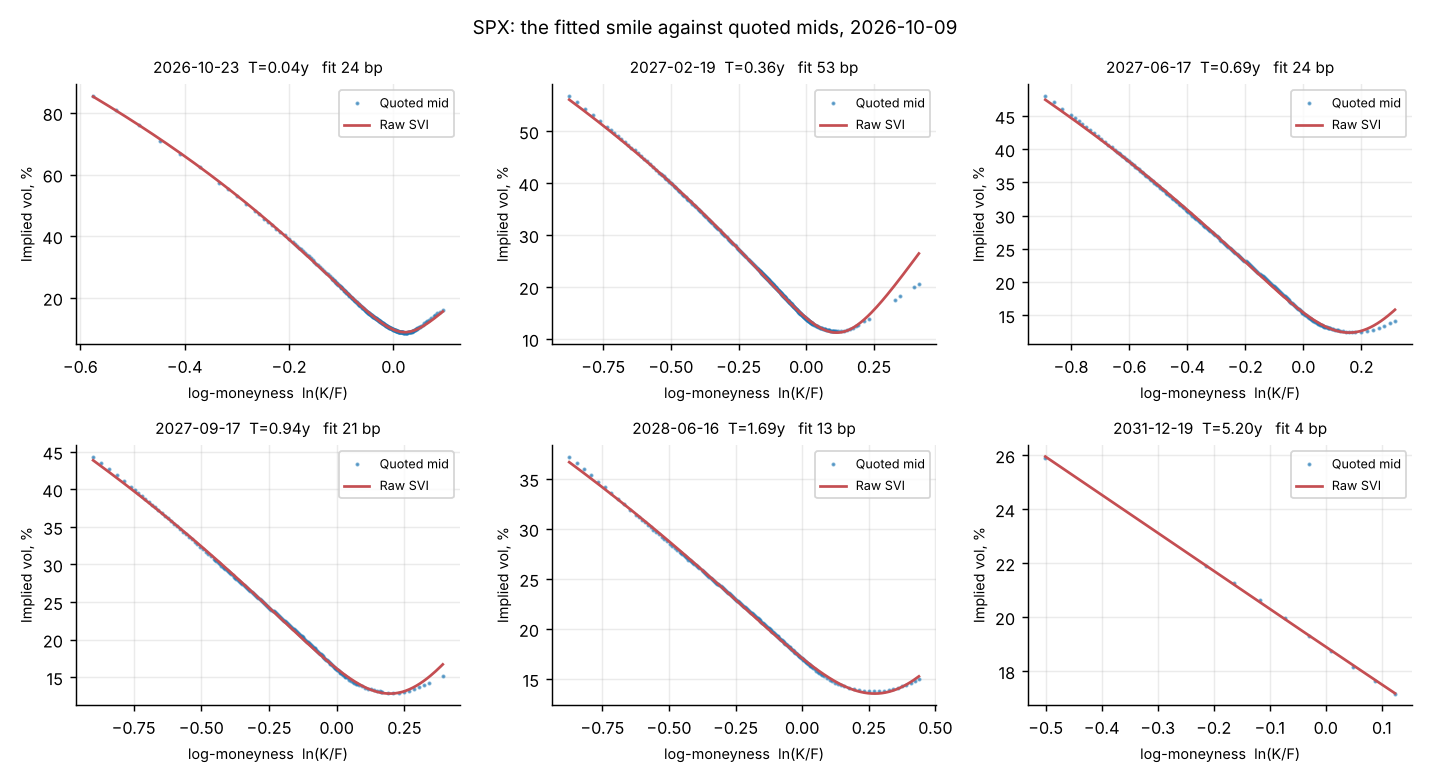
\includegraphics[width=\textwidth]{figures/smile_fits_SPX}
\caption{Fitted S\&P 500 smiles against quoted mids, six expiries from the
9 October 2026 snapshot}
\label{fig:smile}
\notetext{\textit{Notes:} Points are quoted mids, lines the fitted raw SVI
slice. The figure in each panel title is that slice's root-mean-square fit
error in basis points of implied volatility. Panels are ordered by maturity;
the last is the longest listed S\&P 500 expiry at 5.20 years, fitted from ten
quoted volatility points, and each panel plots the quotes falling inside its
own axis range rather than the whole fitted slice. Source:
\texttt{scripts/make\_figures.py}.}
\end{figure}

\section{Results}\label{sec:results}
% Objective: Model values against disclosed values; the funding-spread inversion; the call attribution; the issuer arithmetic that needs no model.

\subsection{Model value against the disclosed value}

\begin{figure}[tbp]
\centering
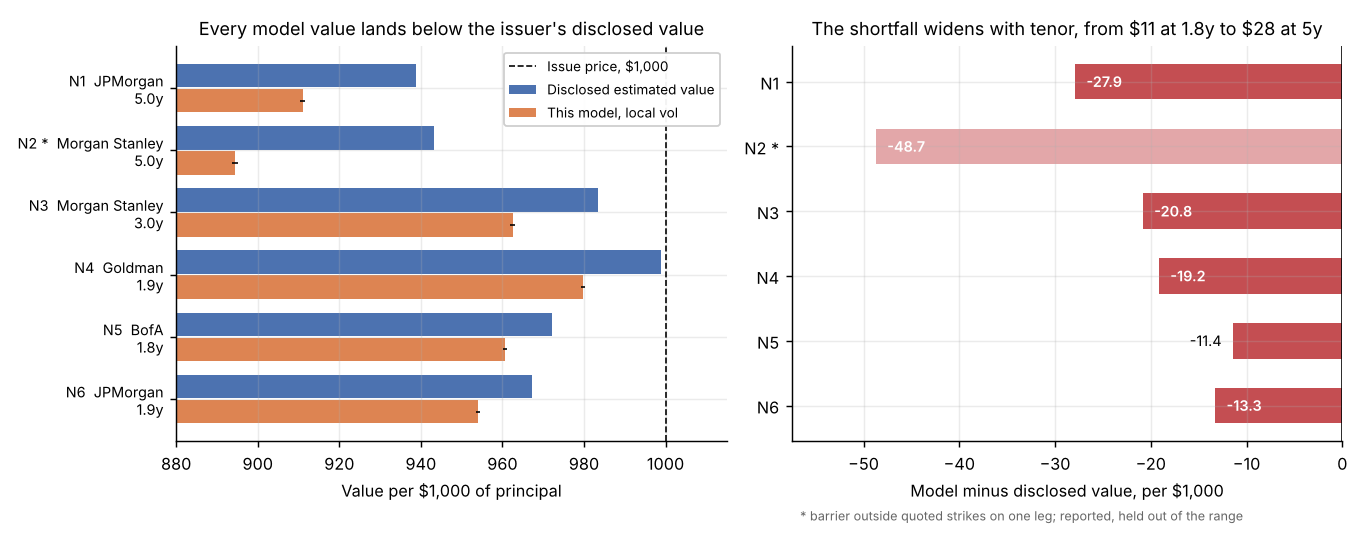
\includegraphics[width=\textwidth]{figures/model_vs_disclosed}
\caption{Model value against the disclosed estimated value, in levels and in
differences, per \$1{,}000 of principal}
\label{fig:gaps}
\notetext{\textit{Notes:} Left panel, the disclosed estimated value and the
model value for each note, with the issue price marked; whiskers are one
standard error of the simulated mean and are smaller than the bar width at this
scale. Right panel, model value less disclosed value. The starred note is
reported but held out of the ranges quoted in the text, for the barrier
coverage reason given in \S\ref{sec:data}. Source:
\texttt{scripts/make\_figures.py}.}
\end{figure}

% Generated by scripts/make_paper_tables.py from the frozen results.
% Do not edit by hand; the next build overwrites it.
\begin{table}[tbp]
\centering
\caption{Model value against the disclosed estimated value, per \$1,000 of principal}
\label{tab:results}
\small
\begin{tabular}{l r r r r r}
\toprule
Note & Model value & s.e. & Disclosed & Gap & Gap (\%) \\
\midrule
N1 & 910.98 & 0.34 & 938.90 & $-$27.92 & $-$2.97 \\
N2\textsuperscript{a} & 894.38 & 0.37 & 943.10 & $-$48.72 & $-$5.17 \\
N3 & 962.56 & 0.29 & 983.40 & $-$20.84 & $-$2.12 \\
N4 & 979.84 & 0.24 & 999.00 & $-$19.16 & $-$1.92 \\
N5 & 960.69 & 0.26 & 972.10 & $-$11.41 & $-$1.17 \\
N6 & 954.01 & 0.30 & 967.30 & $-$13.29 & $-$1.37 \\
\bottomrule
\end{tabular}
\notetext{\textit{Notes:} Model value is the mean discounted payoff over 200,000 paths with a European control variate, at a zero funding spread over the Treasury curve, with the issuer's call exercised by the Longstaff--Schwartz rule. The standard error is of that mean. Gap is model value less disclosed value, so a negative gap means the independent valuation lands below the figure the issuer discloses. Every note shows one. \textsuperscript{a}\,Excluded from the ranges quoted in the text; see Table~\ref{tab:terms}.}
\end{table}


Table~\ref{tab:results} gives the result the rest of the paper is about. Every
model value lands below the issuer's disclosed estimated value. Across the five
notes whose barriers are covered by quoted strikes the shortfall runs from
\$11.41 to \$27.92 per \$1{,}000 of principal, or 1.17 to 2.97 per cent of the
disclosed figure; the note held out of that range is further below still, at
\$48.72. Standard errors are between \$0.24 and \$0.37, so the differences are
one to two orders of magnitude larger than the simulation noise around them.

Figure~\ref{fig:gaps} shows the same thing twice, in levels and in differences.
The ordering in the right panel is worth noting: among the five headline notes
the shortfall increases with tenor, from \$11.41 on the shortest at 1.75 years
to \$27.92 on the longest at 5.00. Five observations do not establish a
relationship and nothing here tests one. But the shape is what a discount-rate
difference would produce, since a constant spread compounds over a longer life,
and that makes the sign of the next result more pointed than it would otherwise
be.

\subsection{The spread that would reconcile them}

% Generated by scripts/make_paper_tables.py from the frozen results.
% Do not edit by hand; the next build overwrites it.
\begin{table}[tbp]
\centering
\caption{The funding spread that would reconcile model and disclosed value, under two assumptions about the call}
\label{tab:spreads}
\small
\begin{tabular}{l r r r r r}
\toprule
Note & Disclosed & Model & Spread (bp) & Model, no call & Spread (bp) \\
\midrule
N1 & 938.90 & 910.98 & -123 & n/a & -1 \\
N2 & 943.10 & 894.38 & -204 & n/a & -69 \\
N3 & 983.40 & 962.56 & -179 & n/a & +76 \\
N4 & 999.00 & 979.84 & no solution & n/a & +99 \\
N5 & 972.10 & 960.69 & -278 & n/a & n/a \\
N6 & 967.30 & 954.01 & -156 & n/a & +121 \\
\bottomrule
\end{tabular}
\notetext{\textit{Notes:} Each spread is the constant addition to the Treasury discount curve that sets the model value equal to the disclosed value, solved on a common set of paths. A funding spread should be positive and wider than the issuer's own senior bonds: the A-rated US corporate option-adjusted spread was 69\,bp on the pricing date. Under optimal exercise every solved spread is negative, from -278\,bp to -123\,bp, which would require the issuer to fund below Treasuries. \textit{No solution} means the disclosed value lies outside the bracket searched; \S\ref{sec:results} reports where that note's crossing lies. The auto-callable note has no no-call column: its redemption is contractual, so removing it describes a different security rather than a different modelling assumption.}
\end{table}


Solving \eqref{eq:inversion} for the funding spread that sets the model value
equal to the disclosed value gives Table~\ref{tab:spreads}. Under optimal
exercise every solved spread is negative, from $-278$ to $-123$ basis points.
The benchmark is 69 basis points, the option-adjusted spread on A-rated US
corporate debt on the pricing date, and an issuer's own funding should sit
above that rather than below it, since a structured note funds more dearly than
a plain senior bond. The solved spreads are on the wrong side of zero, let
alone of the benchmark.

One note returns no solution inside the bracket searched. Extending the grid
for that note alone locates its crossing at $-311$ basis points, 11 basis
points beyond the edge of the bracket, which confirms the absence of a solution
was a property of the search range and not of the note. It changes nothing
about the conclusion: a note whose model value meets its disclosed value only
when the issuer is assumed to borrow 311 basis points below Treasuries is not
reconciled by funding either.

Reading the sign is the whole point. Discounting a liability at a wider spread
lowers its value, so if the disclosed figure were the model value computed with
the issuer's higher internal funding rate, the solved spread would come out
positive. It comes out negative on every note. Whatever accounts for the
difference between these two valuations, a funding rate the filings decline to
publish is not sufficient to be it, and that is the candidate a reader reaches
for first because the filings themselves point there.

The columns for the no-call case show how much of this depends on the exercise
assumption. Removing the issuer's call raises three of the model values above
their disclosed figures, turning those spreads positive. The call, in other
words, is the largest single lever in the model, which is why it gets the next
subsection to itself rather than a sentence here.

\subsection{How much of the call would have to be ignored}

The call assumption can be posed as a quantity rather than a switch. Give the
issuer the funding spread it actually pays, 69 basis points on the pricing
date, and value each note twice: once with the call exercised optimally and
once with no early call at all. The disclosed value's position between those
two bounds is
%
\begin{equation}
  \varphi = \frac{V_{\text{no call}}(\spread) - \mathrm{EV}_{\text{disclosed}}}
                 {V_{\text{no call}}(\spread) - V_{\text{optimal}}(\spread)},
  \label{eq:phi}
\end{equation}
%
the fraction of the call's value that the disclosed figure appears to carry. A
$\varphi$ between zero and one says the disclosed value is consistent with the
issuer pricing some of the call and not all of it. A negative $\varphi$ says
something stronger: the disclosed value sits above the note valued with no call
whatsoever, so no treatment of the call, however generous to the investor,
reaches it at that funding rate.

Three of the five notes to which this applies return $\varphi$ inside the unit
interval, at 0.02, 0.16 and 0.29. For those the disclosed value is consistent
with an issuer recognising between two and twenty-nine per cent of what
optimal exercise is worth, which is a coherent position: a desk may well value
its own call conservatively, and the Morgan Stanley notes' disclosed
rational-exercise rule is itself a weaker commitment than optimality.

The other two return $-1.55$ and $-3.87$. Their disclosed values exceed what
the notes are worth with the issuer's call removed entirely and funding charged
at 69 basis points. Both are the five-year notes. For these the call cannot be
the explanation at any fraction, and the residual has to come from somewhere
else in the model, from a different funding assumption than the corporate
benchmark, or from the disclosed figure itself.

\subsection{What the issuer's own numbers say}

One part of this needs no model at all, only the two figures the issuer prints
on the cover. The gap between the issue price and the disclosed estimated
value is attributed in the filings to the underwriting discount, the expenses
of creating and marketing the notes, and the internal transfer between the
issuing entity and its distribution affiliate (\S\ref{sec:prior}). Subtracting
the disclosed commission from that gap leaves what is available for the other
two components.

On five of the six notes that residual is positive, between \$2.90 and \$20.65
per \$1{,}000. On the sixth it is $-\$4.25$. That note was sold at par with a
disclosed estimated value of \$999 and an underwriting discount of 0.525 per
cent, so net proceeds to the issuer were \$994.75 against a liability the
issuer valued at \$999. The estimated value is quoted to the dollar on that
cover rather than to the cent, so the figure carries about fifty cents of
rounding either way, which does not change its sign.

This is not necessarily an error. The internal transfer component can be
negative if the issuing entity's funding benefit is recognised elsewhere, and
nothing in the disclosure requires the three components to be individually
positive. What it does show is that the disclosed numbers on that cover do not
by themselves decompose into a positive margin, and that the arithmetic is
available to any reader who adds two figures printed a few lines apart.

\subsection{Where the value sits}

% Generated by scripts/make_paper_tables.py from the frozen results.
% Do not edit by hand; the next build overwrites it.
\begin{table}[tbp]
\centering
\caption{The note decomposed into the positions a desk would book, per \$1,000 of principal}
\label{tab:decomposition}
\small
\begin{tabular}{l r r r r r r}
\toprule
Note & Funding bond & Coupon strip & Worst-of put & Issuer's call & Without call & With call \\
\midrule
N1 & 778.77 & 299.87 & $-$135.72 & $-$27.99 & 942.92 & 914.93 \\
N2 & 778.77 & 291.16 & $-$151.68 & $-$22.34 & 918.25 & 895.91 \\
N3 & 864.65 & 234.00 & $-$94.29 & $-$40.09 & 1,004.37 & 964.27 \\
N4 & 913.12 & 171.01 & $-$67.22 & $-$36.38 & 1,016.92 & 980.54 \\
N5 & 920.50 & 90.38 & $-$102.08 & 51.99 & 908.81 & 960.80 \\
N6 & 913.12 & 194.24 & $-$119.14 & $-$34.23 & 988.22 & 954.00 \\
\bottomrule
\end{tabular}
\notetext{\textit{Notes:} The investor is long a funding bond and a coupon strip and short a worst-of put, and signs are from the investor's side. Where redemption is the issuer's decision the call is a cost to the investor and the column is negative. On the one auto-callable note it is positive: redemption is mechanical, returns principal early in states where the note would otherwise stay exposed, and so favours the holder. \textit{Without call} is the sum of the first three columns and \textit{With call} subtracts the fourth. The decomposition runs on 50,000 paths with no control variate, because every part has to be simulated under the same draws for the parts to add up; Table~\ref{tab:results} reports the headline estimator at 200,000 paths with the control variate. The last column is therefore a coarser estimate of the same quantity, not a competing one.}
\end{table}


Table~\ref{tab:decomposition} splits each note into the positions a desk would
book: a funding bond for the principal, a strip of contingent coupons, a short
worst-of put, and the issuer's call. The investor is long the first two and
short the last two. The split is diagnostic rather than a result,
but it locates the magnitudes. After the funding bond the coupon strip is the
largest component on five of the six notes, and the short worst-of put the
largest on the sixth, which is the note with the lowest coupon in the sample.

The call column needs reading with its sign. On the five notes where redemption
is the issuer's decision it is a cost to the investor, between \$22.34 and
\$40.09, and it is of the same order as the \$11 to \$28 to be explained,
which is what makes \eqref{eq:phi} a real question rather than an arithmetic
curiosity. On the auto-callable note it runs the other way, at \$51.99 in the
investor's favour: a mechanical redemption at 93.25 per cent of the initial
level returns principal early in states where the note would otherwise remain
exposed, and the holder gains from it. That is also why \eqref{eq:phi} is not
computed for that note. Its redemption is a contractual term rather than a
discretionary input, so there is no assumption about it to vary.

\section{Which inputs can explain the difference}\label{sec:inputs}

% Generated by scripts/make_paper_tables.py from the frozen results.
% Do not edit by hand; the next build overwrites it.
\begin{table}[tbp]
\centering
\caption{Candidate explanations for the gap, one input at a time, per \$1,000 of principal}
\label{tab:inputs}
\small
\begin{tabular}{l r r r r r}
\toprule
Note & Gap to close & +0.05 correlation & Flat vol & Timing & Call cost \\
\midrule
N1 & $-$27.92 & 9.14 & 62.49 & $-$4.04 & 27.99 \\
N2 & $-$48.72 & 7.70 & 70.21 & $-$7.94 & 22.34 \\
N3 & $-$20.84 & 5.58 & 44.50 & $-$4.56 & 40.09 \\
N4 & $-$19.16 & 3.55 & 31.90 & $-$3.64 & 36.38 \\
N5 & $-$11.41 & 3.32 & 6.65 & $-$3.76 & $-$51.99 \\
N6 & $-$13.29 & 3.10 & 26.71 & $-$4.55 & 34.23 \\
\bottomrule
\end{tabular}
\notetext{\textit{Notes:} Each column is the change in model value from moving one input while the rest are held at their calibrated values, on a common set of paths. \textit{+0.05 correlation} raises every pairwise correlation, confirming the investor is long correlation on every note. \textit{Flat vol} replaces the fitted surface with a single at-the-money volatility per leg. It raises every value, and by more than the gap on five of the six, so the shape of the surface is the one input measured here whose effect both runs toward the disclosed value and is large enough to span the difference. \textit{Timing} aligns the surface to the pricing date rather than the snapshot date and lowers every value, widening the gap. \textit{Call cost} is what the issuer's option to redeem is worth to the issuer, from the decomposition in Table~\ref{tab:decomposition}. No single column closes the gap in the first; \S\ref{sec:inputs} takes them in turn.}
\end{table}

% Objective: Rule candidate explanations in or out one at a time. Correlation, smile, timing, proxy bias, exercise suboptimality.

A candidate explanation has to clear two bars. It must move the model value
toward the disclosed figure rather than away from it, and it must be capable of
moving it far enough. Direction alone is not enough and magnitude alone is
meaningless if the sign is wrong. Table~\ref{tab:inputs} reports each input's
measured effect on a common set of paths, with one input moved at a time and
the rest held at their calibrated values. Taken in turn, four candidates fail
one bar or the other and two survive both. A third survivor sits outside that
table, because it is a dimension the model used here does not have.

\subsection{Ruled out by direction}

Two candidates move the wrong way.

The funding rate was settled in \S\ref{sec:results} and is the first a reader
reaches for, because the filings point there. Raising the discount spread
lowers the model value and widens the gap; closing it requires a negative
spread on every note. Nothing about a funding assumption the issuer declines to
publish repairs that, because the sign is wrong before the magnitude is
discussed.

Observation timing fails the same way. The surface is observed two business
days after five of the notes priced, and aligning it back to each pricing date
using the move in the matching volatility index lowers every value further, by
\$3.64 to \$4.56 across the headline notes. The adjustment is real and it
belongs in the model, but it enlarges the quantity to be explained rather than
reducing it.

\subsection{Right direction, too small}

Two candidates push the right way and cannot reach.

The proxied Dow leg, discussed in \S\ref{sec:data}, raises the affected note by
\$2.61 with a standard error of \$0.73 when corrected on its own. That is about
five per cent of that note's gap, and it touches one note of the six. It is a
real bias with a measured size, and the size is not the size of the problem.

Extrapolating the surface past the longest listed expiry matters only where the
extrapolation is long. Carrying the last observed variance slope forward
instead of freezing the smile raises the five-year note by \$12.36, which is 44
per cent of its gap and far from negligible. On the three notes under two years
the same change is worth \$0.22 to \$0.77. The term structure assumption is
therefore a genuine source of uncertainty on the long end of the sample and
close to irrelevant on the short end, while the gap is present throughout. It
cannot be the common explanation, though it plausibly contributes to the
largest case.

\subsection{Bounded by the exercise policy}

Suboptimal exercise was quantified in \S\ref{sec:results} and the bound it
gives is partial. On three notes the disclosed value sits between the
no-call and optimally-called valuations, consistent with an issuer recognising
two to twenty-nine per cent of the call's worth. On the two five-year notes it
sits above the no-call valuation entirely at a 69 basis point funding spread,
so no exercise assumption reaches it. An explanation that works for three notes
and is arithmetically unavailable for two others is not the explanation,
although it may well be part of the answer for the three.

\subsection{What survives}

Two of the measured inputs clear both bars, and a third candidate clears them
on published evidence without being measurable here at all. None of the three
is published in the filings.

\paragraph{Correlation.} The investor is long correlation on every note, so
raising it raises the model value. The measured sensitivity is \$3.10 to \$9.14
per 0.05 of uniform pairwise correlation. Closing each gap on correlation alone
would take a uniform increase of 0.15 to 0.27, which is three to five times the
perturbation actually measured, obtained by extrapolating a local sensitivity
well beyond the range over which it was computed and therefore an estimate of
the order rather than a precise requirement. The direction is right and there is
a reason to expect a difference: a desk selling a worst-of is short correlation
and marks it above a realised estimate, which is the approximation
\S\ref{sec:method} flagged as the method's largest. Whether the difference is
of this size is not something six notes can settle. The candidate is live and
unresolved.

\paragraph{The shape of the volatility surface.} Replacing each leg's fitted
surface with a single at-the-money volatility raises all six notes, by \$6.65
to \$70.21. This comparison is quoted over all six rather than over the
headline five, because what it measures is a sensitivity rather than a level,
and the barrier-coverage objection of \S\ref{sec:data} bears on the excluded
note's value, not on how that value responds to flattening its surface. On five
of the six the move is larger than the gap: a fully flat surface overshoots the
disclosed value by \$12.64 to \$33.93, and falls short on only one note, by
\$4.87. Somewhere between the quoted smile and no smile at all
there is a surface that reproduces each disclosed figure exactly.

The claim this supports is narrow and the narrowness matters. No desk prices a
worst-of on a flat volatility surface, and nothing here suggests any issuer
did. What the flat-vol valuation provides is a bound: it shows the distance
between this paper's values and the disclosed ones lies inside the range that
disagreement about the shape of the surface can generate, and comfortably
inside it on five notes. A structure whose principal trigger sits 30 to 40 per
cent below the initial level, with coupon barriers 25 to 35 per cent below it,
is priced off the wing of the smile rather than its level, and
the wing is where quotes thin out and modelling choices diverge most. Two
careful desks working from the same quotes can differ there by more than the
amounts in Table~\ref{tab:results}.

\paragraph{The dynamics of that surface.} A third candidate does not appear in
Table~\ref{tab:inputs}, because the model used here cannot produce it. Local
volatility reproduces today's surface and fixes how it evolves; stochastic and
stochastic-local volatility models add a vol-of-vol dimension that a European
repricing gate cannot see. \citet{Farkas2022} put the point sharply for
autocallable barrier reverse convertibles: the stochastic parameters of a
Heston local-stochastic volatility model control the autocallable price
\emph{while leaving the fit to European options unaffected}, and the richer
dynamics typically produce higher prices than local volatility. Higher is the
direction that would close the gap measured here.

Two qualifications stop that from being an answer. Their products are
single-asset and these are worst-of on three underlyings, so the direction is
suggestive rather than transferable. And the candidates are not independent:
\citet{DeCol2017} study equity worst-of autocallables under multi-dimensional
stochastic local volatility and find the correlations between the stochastic
variances central to pricing them, so correlation and volatility dynamics
interact in precisely this product class rather than contributing separately.
Setting them out as two columns of a table, as this section necessarily does,
is itself a simplification.

The consequence for \S\ref{sec:validation} is worth stating plainly. That
section establishes the engine returns the vanilla prices it was calibrated to.
\citet{Farkas2022} establish that two models can agree on every one of those
prices and still disagree on an autocallable. The validation gate is silent on
this dimension by construction, not by oversight.

\subsection{Taken together}

Of the inputs this study can measure, none closes the gap on every note while
moving in the right direction except the shape of the volatility surface, and
that one does so by bounding the problem rather than by identifying a choice.
Funding and timing are excluded by sign. The proxy and the extrapolation are
too small or too narrow. Exercise policy accounts for part of three notes and
none of two. Correlation remains, sufficient in principle at a shift this
sample cannot adjudicate. Beyond what is measured, the dynamics of the surface
remain open, and the published direction favours them.

That is a weaker conclusion than naming a cause and a stronger one than
reporting an unexplained residual. All three surviving candidates are inputs
the disclosure does not contain, and one of them, correlation, is absent even
from the lists of principal inputs that two of these issuers print
(\S\ref{sec:prior}). A reader holding the pricing supplement cannot
distinguish among them, which is a statement about what the disclosure makes
checkable rather than about what any issuer did.

\section{Limitations}\label{sec:limits}
% Objective: Surface two days late; realised not implied correlation; Treasury not OIS; barrier coverage; local volatility's forward skew; six notes.

\subsection{Inputs that are not what a desk would use}

The volatility surface is observed two trading days after five of the six notes
priced, which is a consequence of the filing window in \S\ref{sec:data} rather
than a choice. \S\ref{sec:inputs} measures the cost of that gap, note by note,
and it runs the wrong way to help: correcting for it lowers values further.

Correlation is realised rather than implied, for the reason given in
\S\ref{sec:method}: vanilla options carry no co-movement information and no free
source of implied correlation exists. The bias runs in a known direction, and
\S\ref{sec:inputs} treats it as one of the surviving candidates rather than
burying it here.

Discounting uses the Treasury par yield curve where a dealer would use SOFR
OIS, again because no free source of OIS quotes exists. The two differ by a
handful of basis points at these tenors. That is small against funding spreads
measured in the hundreds, and it is not nothing.

\subsection{The Dow leg, and what the coverage test does not promise}

One leg is priced off fund options standing in for an index
(\S\ref{sec:data}). Two problems follow, and the second is worse than the
first. The level bias is measured at 0.52 volatility points and is worth \$2.61
on the affected note. The more serious problem is that the fund's long-dated
quotes never reach the strike where that note's barrier sits, so for the whole
of its life past the first year the downside is priced off an extrapolation
rather than a quote. That note is reported throughout and excluded from every
quoted range, and its \$0.37 standard error understates its true uncertainty by
an amount this study cannot quantify.

The coverage test that produced that exclusion is a threshold, not a guarantee.
It asks whether a quoted strike exists at or below the trigger on fitted slices
past one year, and a thin market can satisfy it on a single strike while still
pricing the barrier off very little. The other five notes reference index
options deep enough that this is unlikely. Nothing here rules it out.
Appendix~\ref{app:coverage} gives the counts leg by leg so a reader can apply a
stricter threshold.

\subsection{What local volatility does not do}

The engine is calibrated to European option prices and reproduces them, within
the bounds \S\ref{sec:validation} reports. These notes are path-dependent, and
nothing in that validation establishes that local volatility prices the path
dependence correctly. It establishes that the terminal distributions are
right.

This is the model's known weakness rather than an incidental one. Local
volatility reproduces today's surface exactly and misgoverns how that surface
evolves, flattening forward skew in a way that stochastic and stochastic-local
volatility models are built to repair \citep{Qu2016}. It remains market
practice for exotics of this shape because it handles multi-dimensionality,
where stochastic volatility models become expensive to calibrate across several
correlated underlyings \citep{Grzelak2019}. For a worst-of autocallable, whose
value depends on the joint distribution at every observation date and not only
at maturity, the dynamics are a real exposure.

The flat-volatility comparison in \S\ref{sec:inputs} bounds how much the
\emph{shape} of the surface matters. It does not bound how much the dynamics of
that shape matter, and no result in this paper does. What can be said is that
the direction is not unknown: \citet{Farkas2022} report that a Heston
local-stochastic volatility model prices autocallables above local volatility,
with the stochastic parameters moving the autocallable price while the fit to
European options is unchanged. Their products are single-asset. Whether the
same holds for a worst-of on three underlyings, where \citet{DeCol2017} find
the correlations between stochastic variances to be central, is not something
this paper establishes.

\subsection{Exercise, precision and sample}

The issuer's call is solved under optimal exercise, and Longstaff--Schwartz
with a finite basis returns a policy that is suboptimal to some degree. That
error biases the investor's value upward relative to true optimality, so it
pushes the model value toward the disclosed figure and cannot account for a
model that is already too low. The direction is favourable to the finding,
which is worth stating explicitly rather than leaving as an unexamined
approximation.

One issuer discloses its estimated value to the nearest dollar rather than the
cent, so the comparison for that note carries a dollar of irreducible
disclosure precision against a gap of \$19.16. It does not affect the sign of
anything reported.

Six notes, four issuers, one pricing week. Every number here is a case study
and none is an estimate of a population parameter. The 129 final supplements
identified for that week would support a cross-sectional analysis of the
disclosed margin against tenor, coupon, barrier distance and the number of
underlyings. That is left undone, and it is the obvious next thing to do.

\section{Conclusion}\label{sec:conclusion}
% Objective: Answer the question, state both contributions at their true size, name what would settle it.

No. An independent valuation built from public option quotes, a public rates
curve and the terms in the filing itself does not reproduce the issuer's
disclosed estimated value. It lands below it on all six notes, by \$11.41 to
\$27.92 per \$1{,}000 across the five whose barriers are covered by quoted
strikes, against simulation standard errors between \$0.24 and \$0.37.

The funding rate, which the filings themselves name as the input the reader
cannot see, does not account for it. Solving for the spread that would
reconcile the two valuations returns a negative number on every note, from
$-278$ to $-123$ basis points against an A-rated corporate benchmark of 69. The
sign is what carries the result: a disclosed value computed with a higher
internal funding rate would reconcile at a positive spread, and none of them
do.

Taking the remaining candidates one at a time excludes four more. Observation
timing moves values further away. The proxied Dow leg and the choice of term
extrapolation move the right way but are too small, or matter on too few notes,
to be the common cause. Suboptimal exercise accounts for part of three notes
and is arithmetically unavailable for the two five-year ones, whose disclosed
values sit above what the notes are worth with the issuer's call removed
altogether.

Two measured candidates survive on both direction and magnitude. The
correlation assumption would close each gap with a uniform increase of 0.15 to
0.27, which is large but runs the way a dealer's mark is known to run against a
realised estimate. The shape of the volatility surface would close it
comfortably: a fully flat surface overshoots the disclosed value on five of the
six notes. A third candidate cannot be measured with a local-volatility model
at all, and the published direction favours it: \citet{Farkas2022} report that
richer volatility dynamics price autocallables above local volatility, moving
the price while leaving the fit to European options untouched. None of the
three is published in the filing, and one of them, correlation, is not even
named in the lists of principal valuation inputs that two of these issuers
print.

\subsection*{What this paper contributes, and how much}

Two things, both narrower than the subject they sit in.

The first is a verification exercise on the product class the nearest published
work set aside. \citet{Bauer2020} reproduce issuer-disclosed values for German
retail certificates and leave autocallables to later work; this paper prices
six of them from public inputs and reports the funding-spread inversion as a
diagnostic, which converts an unexplained difference into a statement about
what the difference cannot be. The result is a case study on six notes from one
week, not an estimate of anything about the market. Whether these gaps are
typical is unknown, and nothing here should be read as suggesting they are.

The second is a census of what the exercise can reach at all. Of 1{,}086
supplements filed on Form 424B2 in the sample week, 129 are final worst-of
notes with a contingent coupon and a disclosed estimated value, and 71 of those
can be priced from public option quotes. A reader checking this disclosure can
therefore reach 55 per cent of the qualifying market, and the inaccessible
remainder is not a random sample of it: 33 of the 42 notes excluded for
unlisted options reference a single US sector index that has no options market
of its own. That bound is a fact about the disclosure regime rather than about
any issuer, and it would hold for any outside party attempting the same check.

\subsection*{What would settle it}

None of the three surviving candidates requires access to an issuer's models to
test. Two of them, though, are not cleanly separable from each other, which
shapes the order the tests should be run in.

Correlation could be tested directly with dispersion trade data or with quotes
on multi-asset structures from which an implied correlation can be backed out.
If dealer correlation marks on these underlyings sit 0.15 to 0.27 above the
realised estimate over the relevant horizon, correlation is sufficient on its
own and the question becomes how much of the gap it takes. If they sit much
closer, it is not.

The surface dynamics could be tested by repricing the same six notes under a
stochastic-local volatility model calibrated to the same quotes. The
single-asset version of that test has been run: \citet{Farkas2022} find a
Heston local-stochastic volatility model prices autocallables above local
volatility, with the stochastic parameters moving the price while the European
fit is untouched. What is missing is the multi-asset case, where
\citet{DeCol2017} find the correlations between stochastic variances to be
central, and where the dynamics candidate and the correlation candidate stop
being separable. Running it on these six notes would show whether the residual
reported here survives a model that can see the dimension this one cannot.

The sample is the third thing to extend, and the cheapest. The 129 final
supplements identified for one week would support a cross-sectional analysis of
the disclosed margin against tenor, coupon, barrier distance and the number of
underlyings, and the screening code that produced them runs forward on any
later week. Whether the pattern reported here survives contact with a hundred
notes rather than six is the question this paper cannot answer and the one most
worth asking next.

% Unnumbered back matter, in the same set and the same order as the author's
% previous working paper.
%
% Two departures from that template, both deliberate. The availability
% statements are written for this project rather than carried over: the earlier
% paper rested on licensed vendor records it could not redistribute, while every
% input here is public and the repository is public with it. And the earlier
% paper's "Code availability" heading carried a sentence about data, which is
% repaired rather than reproduced.
%
% The generative-AI-use declaration keeps the earlier paper's wording and
% position, with the tool named as the one actually used. scripts/
% scan_repository.py lists this section as a documented exception to the
% repository's vocabulary check.

\section*{Funding}
The author declares no external funding.

\section*{Disclosure statement}
The author declares no competing financial interests.

\section*{Data availability statement}
Every input to this study is public. The six pricing supplements are preserved
in full under \texttt{references/sec\_filings/} and remain retrievable from
EDGAR under the accession numbers recorded in
\texttt{references/source\_register.csv}. Option quotes are delayed end-of-day
chains from Cboe's public endpoint, captured on 9 October 2026. The eight chains
the reported results depend on are tracked in the repository alongside the
SHA-256 digest of each file, so a reader can confirm that the surfaces were
fitted to the quotes recorded here rather than to a later capture. The other
chains taken that morning are not tracked, and since the endpoint serves only
current quotes they cannot be retrieved for that date afterwards. The Treasury
par yield curve, the Cboe volatility index histories and the FRED series are
published by the issuing institution and are downloaded by
\texttt{scripts/fetch\_reference\_data.py}. Daily closes for the one
exchange-traded fund among the underlyings come from a commercial endpoint
rather than an official series, which is noted where that note is priced.

\section*{Code availability}
The pricing engine, the calibration code, the test suite and the frozen outputs
behind every number reported here are available at
\url{https://github.com/soham-parundekar/autocallables-notes-pricing}. The Monte
Carlo results reproduce exactly rather than approximately: the path count and
the seed are recorded in \texttt{config/params.yaml}, and \texttt{make surfaces
validate analysis report} regenerates the calibrated surfaces, the tables and
the figures from the preserved snapshot. The repository was cloned into a clean
environment and that sequence rerun before the results were frozen, which
returned the calibrated parameters to the last digit and the reported tables
byte for byte.

\section*{Declaration of generative AI use}
During the preparation of this work, the author used Claude in order to revise
and restructure the manuscript, prepare the plotting script, literature checks
and LaTeX preparation. After using this tool/service, the author reviewed and
edited the content as needed and takes full responsibility for the content of
the published article.




\begingroup
\small
\setlength{\bibsep}{4pt}
\bibliographystyle{apacite}
\bibliography{references}
\endgroup

\appendix
\section{Term sheet detail for the six notes}\label{app:terms}

Each note is identified below by CUSIP and by the EDGAR accession number of the
priced supplement it was read from. All six documents are preserved in full in
the project repository, and all six remain retrievable from EDGAR under these
accession numbers. The economic terms appear in Table~\ref{tab:terms}; what
follows is the information needed to locate the source and to see which
structural variant each note is.

\begin{table}[htbp]
\centering
\caption{Filing identifiers and structural variant}
\label{tab:filings}
\small
\begin{tabular}{l l l l l}
\toprule
Note & CUSIP & Accession number & Coupon frequency & Redemption \\
\midrule
N1 & 46661PD38 & 0001918704-26-031125 & monthly   & issuer's option \\
N2 & 61781LWY2 & 0001839882-26-050390 & monthly   & rational-exercise rule \\
N3 & 61781LM23 & 0001839882-26-050393 & monthly   & rational-exercise rule \\
N4 & 40058M7F9 & 0001193125-26-419171 & monthly   & issuer's option \\
N5 & 09712CWN9 & 0001918704-26-030916 & quarterly & automatic at 93.25\% \\
N6 & 46661PL96 & 0001918704-26-031101 & monthly   & issuer's option \\
\bottomrule
\end{tabular}
\notetext{\textit{Notes:} Product names as printed on the covers are
\textit{Callable Contingent Interest Notes} (N1, N6), \textit{Callable
Contingent Income Securities} (N2, N3), \textit{Callable Contingent Coupon
Index-Linked Notes} (N4) and \textit{Contingent Income Auto-Callable Yield
Notes} (N5). Each note is issued by a finance subsidiary and guaranteed by its
parent. The three notes redeemable at the issuer's option become redeemable on
scheduled payment dates after an initial non-call period: from the twelfth
payment date on N1 and from the third on N4 and N6, in each case excluding the
final payment. The two governed by the rational-exercise rule are redeemable on
every stated redemption date, 48 of them on N2 and 30 on N3.}
\end{table}

One structural difference matters for the simulation and is not visible in
Table~\ref{tab:terms}. Five of the notes observe the downside trigger only at
maturity, so a breach is a European condition on the terminal level. The
auto-callable note observes it on any trading day, which is an American
knock-in and is handled in the simulation by a per-path indicator updated at
every daily step rather than at the observation dates alone.

\section{SVI calibration and the arbitrage conditions}\label{app:svi}

\subsection*{The fit}

Fitting all five raw parameters of \eqref{eq:svi} at once is possible and
unreliable. The objective has local minima, and on the S\&P 500 expiry at
$T = 0.36$ a direct least-squares run in this sample converged to
$\rho = +0.39$, a positive skew, which is the wrong sign for an equity index
and left 26 basis points of error at the money.

The fit used here is the quasi-explicit reduction. The reduction itself
predates the arbitrage-free treatment, having been proposed in a 2009
whitepaper that \citet{MartiniMingone2022} record as its origin; it is their
paper that characterises which reduced parameters correspond to an
arbitrage-free slice, which is what makes a constrained refit well posed.
Substituting
$y = (\logm - m)/s$ turns \eqref{eq:svi} into
%
\begin{equation}
  \totvar(y) = a + (b\,\rho\,s)\,y + (b\,s)\sqrt{y^2 + 1},
  \label{eq:svi-reduced}
\end{equation}
%
which is linear in the three coefficients $(a,\; c = b\rho s,\; d = bs)$. The
outer search therefore has to handle only $m$ and $s$, with the inner problem
solved exactly as a weighted linear least squares at each candidate pair. Two
constraints make the solution a valid slice: $d \geq |c|$, which is $|\rho| \leq
1$, and $a + \sqrt{d^2 - c^2} \geq 0$, which keeps total variance non-negative
everywhere. The unconstrained inner solution usually satisfies both, and the
constrained solver runs only when it does not, which is what keeps the
two-dimensional outer search affordable.

\subsection*{The weighting, and why it is not uniform}

Residuals are measured in total variance, but the quantity that matters is
error in implied volatility, and the two objectives are not the same. On the
fitted S\&P 500 slice at $T = 0.94$, total variance runs from 0.0245 at the
money to 0.1546 at the deepest quoted strike, a factor of 6.3. Least squares
weights by the square of the residual, so an unweighted fit in $\totvar$ is
dominated by the wing at roughly 40 to 1 and will fit the tail at the expense
of the strikes that matter most for a note struck near the money.

Since $d\totvar = 2\sigma T\, d\sigma$, scaling each weight by
$1/(2\sigma T)^2$ converts the objective into squared volatility error while
leaving it linear in the coefficients, which is what the reduction in
\eqref{eq:svi-reduced} requires. That factor multiplies a base weight taken
from quote tightness, the reciprocal of the relative bid-ask, capped at 50 so
that one unusually tight quote cannot dominate its slice.

\subsection*{Enforcing the two conditions}

The butterfly condition \eqref{eq:butterfly} is evaluated after each fit on a
grid scoped to that expiry's own quoted strikes, padded by 0.10 in
log-moneyness and capped at five standard deviations of total volatility. A
slice violating it anywhere on that grid is refitted with the condition
imposed, rather than having the offending wing smoothed afterwards.

The calendar condition is enforced pairwise between adjacent fitted expiries on
the grid they share. Where total variance decreases in maturity at any point,
the later slice is refitted subject to
$\totvar_{\text{later}}(\logm) \geq \totvar_{\text{earlier}}(\logm)$. Expiries
closer than 25 days apart are thinned beforehand, because two nearly coincident
expiries divide independent fit error by a very small $\Delta T$ and manufacture
violations that are an artefact of the spacing rather than a property of the
surface.

Grid scope is not a detail. Enforcing these conditions on a single wide grid
spanning $\logm \in [-1.5, 1.0]$ asks a two-week slice about strikes far beyond
anything it quotes, where it is purely extrapolating, and the calendar
condition then makes that extrapolated wing a floor for every later expiry. The
constraint propagates forward from the slice with the least information rather
than the most, and the degradation compounds across the term structure. Scoped
instead to the strikes each pair of adjacent expiries actually quotes, the
surfaces fit without that pressure, and the audit in \S\ref{sec:validation}
returns zero failures of either condition across all 68 slices.

\section{Quoted strike coverage at each note's barrier}\label{app:coverage}

A worst-of note's entire downside sits at its trigger, so the surface is queried
there far more consequentially than at the money. Whether a quote exists at that
point separates interpolating the smile from extrapolating it, and the
distinction decides which notes carry ranges quoted in the text.

Table~\ref{tab:coverage} counts, for every leg of every note, the fitted slices
with maturity beyond one year whose quoted strikes reach down to the note's
trigger. One year is the threshold because the short end of every surface here
is quoted deep enough for the question not to arise. A leg scoring zero prices
that note's downside, for the whole of its life past the first year, from an
extrapolated wing.

One leg of one note scores zero. That note is reported throughout and held out
of every range quoted in \S\ref{sec:results} and \S\ref{sec:inputs}. The rule
is stated as a count rather than a verdict so that a reader who considers the
threshold too lenient can apply a stricter one without re-running anything:
requiring coverage on a majority of deep slices rather than on one, for
instance, changes no note's status in this sample.

% Generated by scripts/make_paper_tables.py from the frozen results.
% Do not edit by hand; the next build overwrites it.
\begin{table}[htbp]
\centering
\caption{Quoted strike coverage at each note's downside trigger, by leg}
\label{tab:coverage}
\small
\begin{tabular}{l r l c}
\toprule
Note & $\logm$ at trigger & Covered slices past one year, by leg & Fully covered \\
\midrule
N1 & $-$0.431 & NDX 2/2, RUT 3/3, SPX 8/8 & yes \\
N2 & $-$0.431 & DJX 0/5, NDX 2/2, RUT 3/3 & \textbf{no} \\
N3 & $-$0.511 & NDX 2/2, RUT 3/3, SPX 8/8 & yes \\
N4 & $-$0.511 & NDX 2/2, RUT 3/3, SPX 8/8 & yes \\
N5 & $-$0.357 & NDX 2/2, RUT 3/3, SPX 8/8 & yes \\
N6 & $-$0.511 & RUT 3/3, SMH 5/5, SPX 8/8 & yes \\
\bottomrule
\end{tabular}
\notetext{\textit{Notes:} The trigger is expressed as log-moneyness relative to the initial level, so $-0.431$ is a trigger at 65 per cent of it. For each leg the entry counts the fitted slices with maturity beyond one year whose quoted strikes reach down to that level, against the number of such slices. A leg at 0 prices that note's entire downside past the first year from an extrapolated wing rather than from a quote. One note fails on one leg and is held out of every range quoted in the text, though its own figures are reported throughout.}
\end{table}



\end{document}
